\chapter{Fundamentação Teórica}
\label{cap:fundamentacao}
Neste capítulo serão abordados os principais conceitos e tecnologias utilizadas no desenvolvimento deste projeto, do hardware à aplicação móvel, iniciando pelo conceito principal, a Internet das Coisas.

% ---
\section{Internet das Coisas}
\label{fund:iot}
Com o intuito de ampliar a internet atual, interligando os objetos do nosso cotidiano, animais e humanos em uma única rede, foi criado a Internet das Coisas, IoT, também conhecida como internet de todas as coisas. Para tal, os objetos viram objetos inteligentes, possuindo capacidade de comunicação associados com sensores que fornecem dados para outros dispositivos. Estes aparelhos, conectados a IoT, se comunicam via internet, trocando dados em tempo real, transmitindo informações acerca do ambiente que estão inseridos e/ou até mesmo dos seus respectivos estados. 

Deste modo, é adicionada uma nova gama de possibilidades, trazendo grandes benefícios para ambientes domésticos, mas principalmente para a área industrial. No primeiro caso, aplicações, tais como: aprendizagem reforçada, monitoramento e vigilância inteligentes e vida assistida, têm despontado entre aquelas que mais chamam atenção, tanto dos usuários, como das empresas de desenvolvimento de soluções tecnológicas. No segundo caso, IoT se apresenta como um diferencial competitivo importante em campos, com a automação e manufatura industrial, logística, gestão de processos de negócio, entre outros.

Do ponto de vista da produtividade, IoT apresenta-se como um importante meio pelo qual pode-se desenvolver aplicações sofisticadas que podem integrar o mundo real e o mundo virtual. Em empresas de manufatura, produtos conectados permitem a existência de um ambiente de serviços e produtos no qual a manutenção pode ser realizada com base na necessidade real, em vez de uma suposição estatística. Adicionalmente, produtos e máquinas conectados podem receber atualizações de software quando disponíveis, para garantir que estejam sempre funcionando em eficiência ótima.

Entretanto, a IoT enfrenta grandes desafios na sua implantação, tanto na transmissão de dados quanto na autonomia energética. No ambiente residencial, paredes e dispositivos eletrônicos se tornam obstáculos para os dispositivos da IoT, na área industrial, esses empecilhos são mais presentes, devido a grande concentração de equipamentos metálicos. Outros problemas, fora os causados pelo ambiente, são devido a grande concentração de tais dispositivos transmitindo simultaneamente, que podem acabar gerando interferência. Ademais, há um grande número de dispositivos que não podem ficar conectados na energia elétrica por cabos, por razões variadas, e, graças a sua quantidade, é preciso que  durem por um grande período de tempo com a mesma fonte de energia para tornarem-se viáveis, pois, gerenciar as baterias usadas por inúmeros dispositivos em uma grande frequência, acaba sendo custoso. Tendo esses pontos em mente, algumas tecnologias foram criadas para tal finalidade, entre elas uma das que mais se destacam é a LoRa.

A tecnologia Long Range, LoRa, é uma forma de comunicação sem fio, semelhante ao Wi-Fi e ao Bluetooth, que permite um longo alcance de comunicação com baixo custo. O raio de comunicação sem fio utilizando o LoRa, dependendo do dispositivo selecionado, pode alcançar quilômetros de distância.

Embora o LoRa tenha sido fundamentalmente desenvolvido pela Semtech Corporation, seu padrão imposto pelo LoRa permitiu que muitas empresas a utilizassem para diversos projetos com um custo benefício satisfatório, aumentando o ecossistema e ganhando um envolvimento significativamente maior, uma variedade superior de produtos e um acréscimo geral no uso e aceitação. 

O LoRa em si diz respeito à camada física, sendo a camada lógica chamada de LoRaWAN, um protocolo usado pelo LoRa para comunicação entre pontos de conexões de um nós finais (\textit{End Nodes}) para envios de informações diretamente a um concentrador (\textit{Gateway}), que centraliza as informações e envia a um determinado sistema \cite{lora2021specification}. Os End Nodes são dispositivos responsáveis por coletar os dados necessários e transmiti-los a um determinado Gateway, o Gateway por sua vez, é responsável por receber as informações de múltiplos End Nodes e repassá-las a um determinado sistema, por exemplo um servidor onde os dados serão armazenados, como podemos ver na figura \ref{fig:end-nodes-gateways}.

\begin{figure}[H]
  \centering
  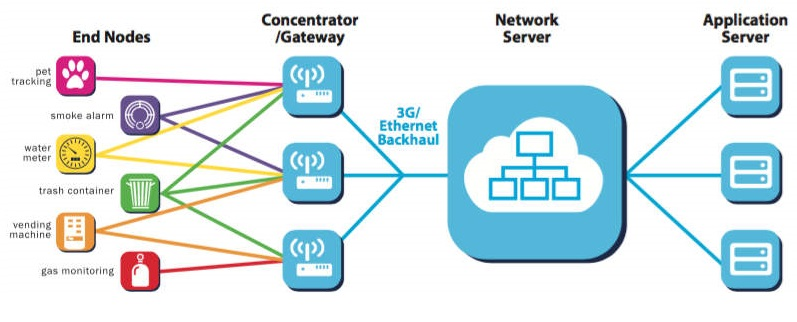
\includegraphics[width=.80\textwidth]{assets/lora-network-architecture.png} 
  \caption{Representação da relação entre os dispositivos LoRa (Adaptada de \cite{lora2021architecture}).}
  \label{fig:end-nodes-gateways} 
\end{figure}

% ----
% \subsection{HTTP/HTTPS}
% \label{fund:http}
% Inicialmente utilizado pelo \textit{World-Wide Web}, WWW, em 1990, como o protocolo base da internet por ser um protocolo leve e rápido para transmissão de informações em sistemas distribuídos, o \textit{Hypertext Transfer Protocol}, HTTP, é um protocolo que transmite documentos de diversos formatos através de sistemas distribuídos, mais conhecido pela sua disseminação pela internet \cite{berners1996hypertext}. Quatro anos depois, em 1994, a Netscape Communications criou o HTTPS, uma implementação do HTTP adicionando uma nova camada, a de segurança, utilizando-se do protocolo SSL/TLS, um protocolo que fornece segurança entre comunicações sobre rede de computadores.

% O HTTP funciona baseado no paradigma de cliente e servidor, onde o cliente estabelece uma conexão fazendo uma requisição solicitando algo ao servidor, e o servidor, por sua vez, o responde enviando uma mensagem.  Tais requisições possuem um método atrelado a ele, esses métodos são usados semanticamente, com o objetivo de organizar e dividir suas responsabilidades, os métodos mais utilizados são: GET, POST, PUT e DELETE. o GET é usado quando o cliente solicita dados ao servidor, o POST quando o cliente quer enviar alguma nova informação, o PUT é semelhante ao POST, entretanto, é referente a atualização de um dado existente e o DELETE é uma requisição pedindo a remoção de uma determinada informação \cite{mozilla2019http}.

% Essas mensagens que transitam entre clientes e servidores são compostas por linhas de textos divididas em três blocos como pode ser visto na figura \ref{fig:post-request}. O primeiro bloco consiste em uma linha com o método da requisição, a url, ou seja, o caminho do documento seguido pela a versão do protocolo; o segundo bloco é referente ao cabeçalho HTTP, responsável por fornecer informações e metadados ao servidor, como o tipo de dado transitado ou dados que alteram seu comportamento; o terceiro bloco diz respeito ao bloco de dados. Este bloco é opcional, dependendo do tipo de requisição realizada, mais utilizado pelos métodos POST e PUT.

% \begin{figure}[H]
%   \centering
%   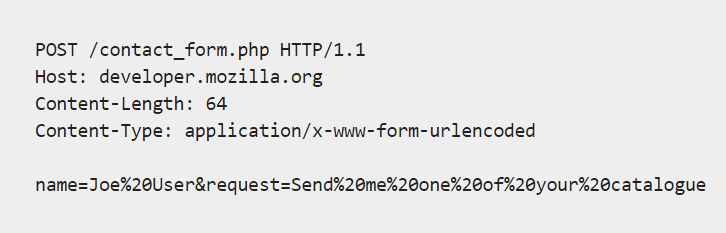
\includegraphics[width=.80\textwidth]{assets/post-request.png} 
%   \caption{Exemplo de uma requisição POST (Retirado de \cite{mozilla2019http}).}
%   \label{fig:post-request} 
% \end{figure}

% ---
% \section{Plataformas de Prototipagem}
% \label{fund:plataforma-proto}
% Plataformas de prototipagem eletrônica são formas facilitadas de desenvolver um protótipo inicial de determinado projeto. Uma das plataformas de prototipagem existentes mais famosa é o Arduino, uma plataforma de código aberto criada em 2005 na Itália pelo professor Massimo Banzi, que tinha como objetivo, ensinar eletrônica e programação para seus alunos, provendo uma forma acessível e de fácil uso. O Arduino possui seu próprio ambiente de desenvolvimento de mesmo nome, utilizando de sua linguagem de programação baseada em C.

% Outra plataforma bem conhecida é a família de microcontroladores ESP, e assim como suas concorrentes, oferece módulos de baixo custo e versáteis para várias soluções tecnológicas, dos quais destacam-se a série ESP32. Tal série, acabou sendo mais conhecida pelas suas variações de modelos feitas por empresas distintas, cada modelo possuindo seus diferenciais, como por exemplo o modelo da Heltec Automation, que inclui conectividades com WiFi, bluetooth e LoRa.

% ---
\section{Sensor DHT-22}
\label{fund:dht-22}
O sensor DHT-22 é um sensor de temperatura e umidade da família de sensores DHT comumente utilizado em aplicações de IoT por ser um sensor pequeno(como podemos ver na figura \ref{fig:dht-22}) e possuir um baixo custo. Ele opera na faixa de 3.3 a 6 Volts e consegue capturar dados de temperatura entre -40°C a 80°C e umidade entre 0\% a 100\% RH, com uma acurácia de 0.5°C e 2\% RH, respectivamente \cite{datasheetDHT22}.

\begin{figure}[H]
  \centering
  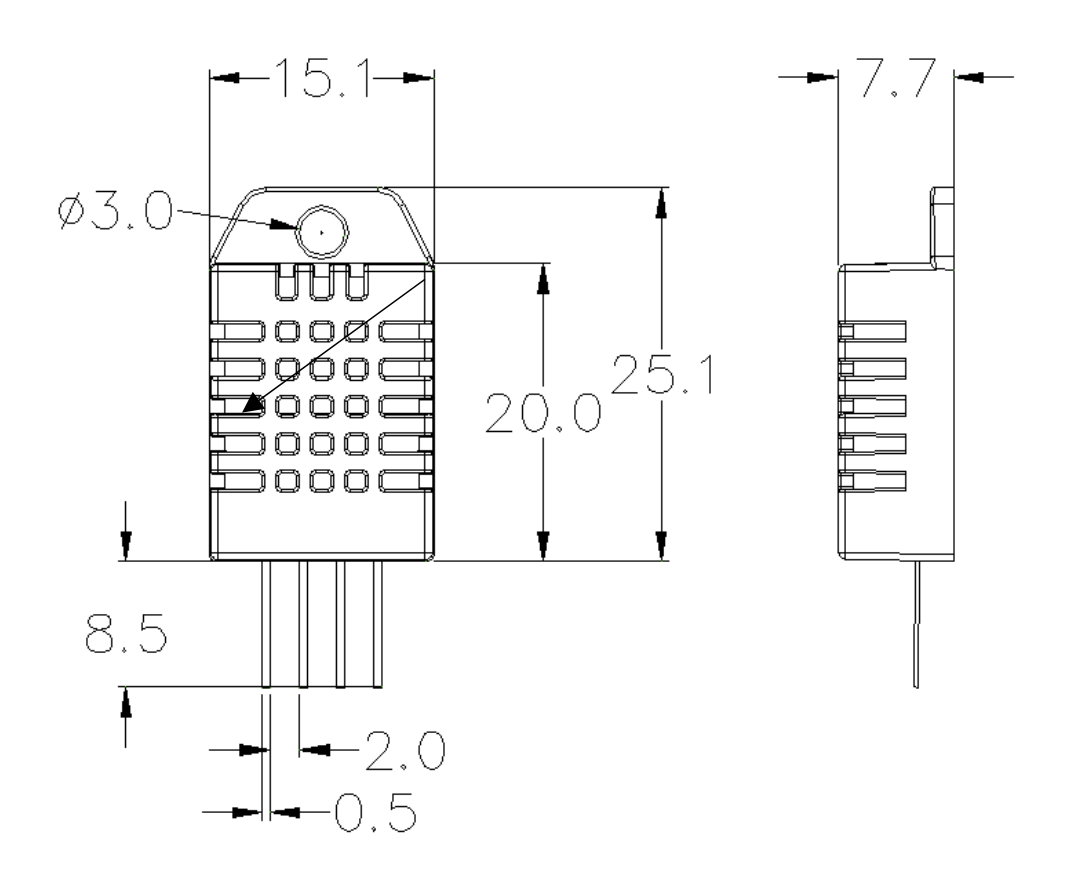
\includegraphics[width=.80\textwidth]{assets/dht-22.png} 
  \caption{Dimensões em milímetros do sensor DHT-22 (Retirado de \cite{datasheetDHT22}).}
  \label{fig:dht-22} 
\end{figure}

% ---
\section{Servidor}
\label{fund:servidor}
Um servidor é um sistema de computação centralizada, responsável por fornecer serviços em uma rede de computadores. Esses serviços variam conforme a necessidade do sistema, podendo ser um controlador de domínio, provedor de arquivos, de impressão, de e-mails entre outros. No modelo cliente/servidor (figura \ref{fig:client-server-model}), por sua vez, o servidor é responsável por receber as requisições de clientes, provendo informações e dados de acordo com a demanda.

\begin{figure}[H]
  \centering
  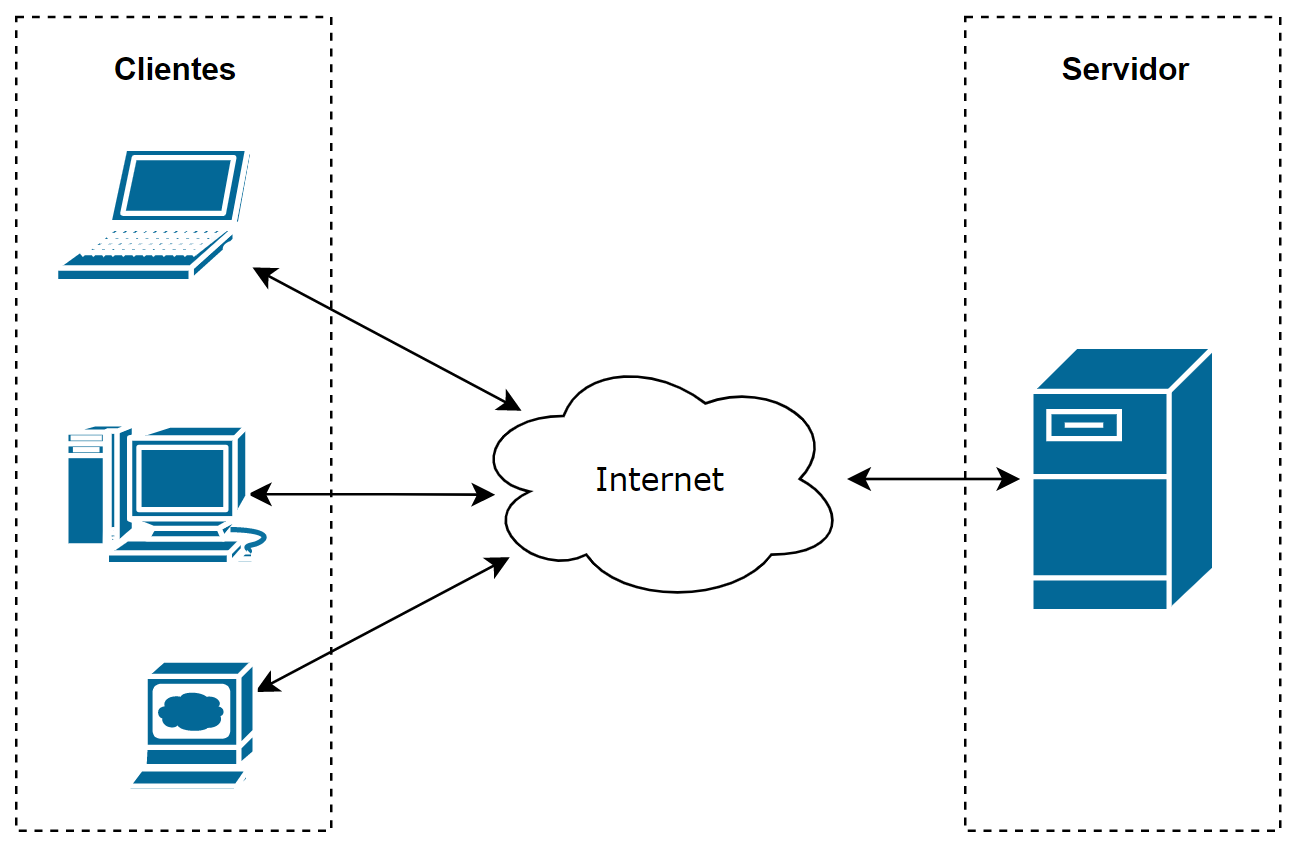
\includegraphics[width=.80\textwidth]{assets/client-server-model.png} 
  \caption{Representação do modelo cliente/servidor (Autoral).}
  \label{fig:client-server-model} 
\end{figure}

% ----
\subsection{Node.js}
\label{fund:node}
Em 2009, Ryan Dahl criou o Node.js ou simplesmente Node, um ambiente de código aberto de execução Javascript para ser utilizado por servidores (\textit{server-side}) baseado no interpretador V8 da Google. O objetivo do Node é fornecer uma forma de criar serviços com alta capacidade de escala, consumindo pouca memória e de fácil aprendizado. Apesar da linguagem de programação Javascript fornecer uma performance inferior às linguagens já existentes para esse objetivo, seu uso oferece dois grande benefícios, ser uma linguagem de fácil aprendizado e de grande uso por ser a linguagem padrão dos navegadores, e consequentemente do desenvolvimento web \cite{tilkov2010node}.

A forma de execução no Node é por eventos assíncronos, diferente da maioria dos outros ambientes modernos que utilizam \textit{threads} do sistema operacional, SO. O Node usa apenas uma thread assíncrona principal que executa operações de entrada e saída de dados, E/S, chamada de \textit{Event Loop}, em português, ciclo de eventos \cite{nodejsAbout}. O \textit{Event Loop} funciona em um ciclo, escutando uma lista de chamadas, onde são armazenadas as requisições recebidas, e as direcionando cada uma para uma Thread a parte, que executará a função recebida, como podemos ver na figura \ref{fig:event-loop-node}. A priori, o  Node possui quatro \textit{threads} trabalhadoras, responsáveis por executar as funções. Entretanto, é possível configurar a quantidade de \textit{threads} usadas, dependendo da máquina, onde está sendo efetuado a instância do Node.

\begin{figure}[H]
  \centering
  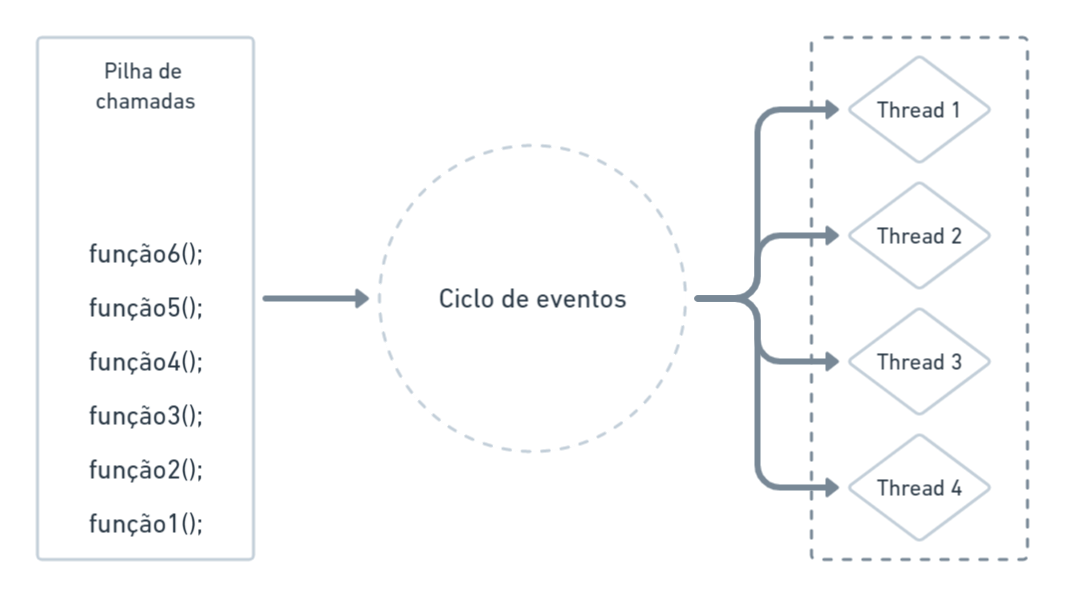
\includegraphics[width=.80\textwidth]{assets/event-loop-node.png} 
  \caption{Ciclo de eventos no Node (Autoral).}
  \label{fig:event-loop-node} 
\end{figure}

% ----
\subsection{InfluxDB}
\label{fund:influxdb}
O InfluxDB é um banco de dados que armazena séries temporais (\textit{data series database}), ou seja, sua chave é o tempo e sua forma de armazenagem de dados é em ordem cronológica. Ele foi projetado para lidar com grandes cargas de escrita e consulta, perfeito para armazenar dados em tempo real, como monitoramento de DevOps, métricas de aplicativos, big data e dados de sensores da IoT \cite{giacobbe2018implementation}. De forma geral, séries temporais acabam se tornando gráficos em função do tempo em um determinado período, por exemplo a temperatura de um freezer ao decorrer do dia, podendo assim ver facilmente a máxima, a mínima e suas variações. Esses dados podem ser também coletados e feito uma análise mais complexa usando qualquer ferramenta estatística, dependendo da sua necessidade.

O InfluxDB é composto por \textit{databases} (bancos de dados), \textit{measurements} (medições), \textit{fields} (campos) e \textit{tags}. Podemos representar essa estrutura como conjuntos como podemos ver na figura \ref{fig:influxdb-struct}. No InfluxDB é possível ter inúmeros \textit{databases}, onde cada \textit{database} contém suas \textit{measurements} que são tabelas de dados correspondentes a algum dado em específico. Por exemplo, se tivermos 2 sensores que coletam dados diferentes, cada sensor viraria um \textit{measurement}, e cada \textit{measurement} é composto  de dois tipo de atributos, os \textit{fields}, onde ficam os dados da sua medida, e as \textit{tags}, que são campos de dados que diferem \textit{fields} por serem campos indexáveis, feitos exclusivamente para realizar buscas, tal como, é comum adicionar uma \textit{tag} que seja um identificador do dispositivo que coletou esse medida.

\begin{figure}[H]
  \centering
  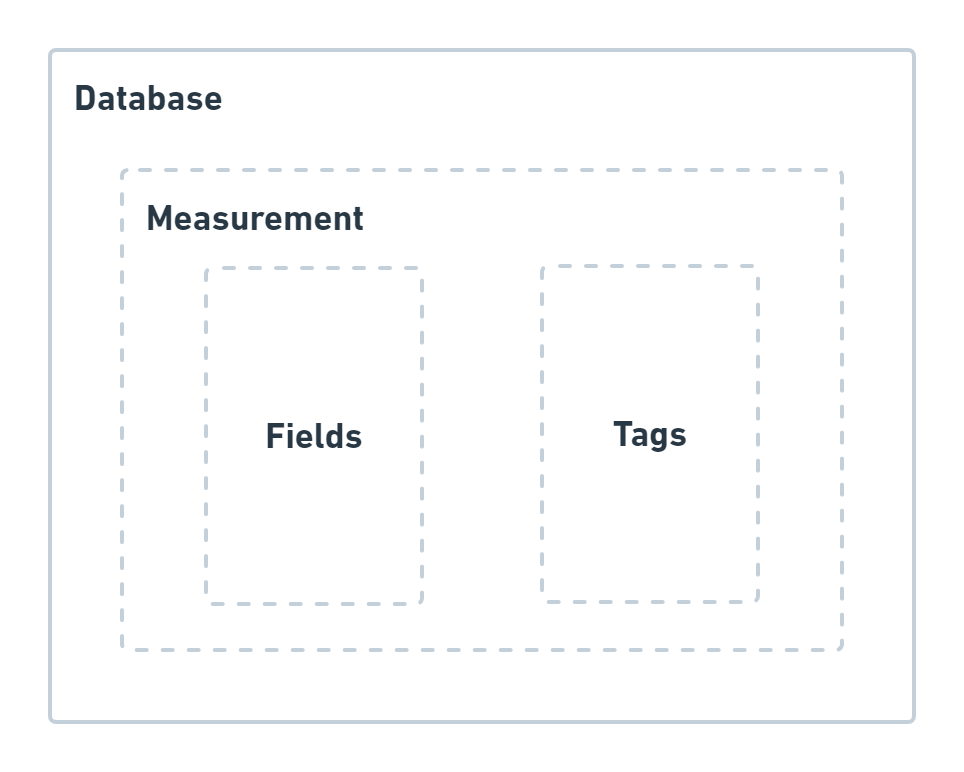
\includegraphics[width=.80\textwidth]{assets/influxdb-struct.png} 
  \caption{Organização dos dados no InfluxDB (Autoral).}
  \label{fig:influxdb-struct} 
\end{figure}

% ----
\subsection{Docker}
\label{fund:docker}
Docker é uma plataforma \textit{open source}, desenvolvida utilizando a linguagem de programação GO pela Google, com o objetivo de criar facilmente  ambientes isolados (containers) com um alto desempenho e portáteis, sendo uma opção em relação às virtualizações. Desta maneira, é possível, por exemplo, criar inúmeras aplicações usando as mesmas tecnologias, cada uma em um \textit{container} diferente e nenhuma vai interferir na outra, e todas na mesma máquina. Se for preciso replicar em outra máquina, é possível criar uma imagem do container e instalar o mesmo ambiente nesta outra máquina.

Em comparação com as virtualizações, os containers não precisam de um sistema operacional, apenas o essencial para executar determinada função. Dessa forma, os containers conseguem ter um controle maior, consomem menos recursos, ganham uma maior flexibilidade e manutenibilidade. Podemos ver a comparação entre virtualização e containers na figura abaixo.

Apesar dessa facilidade que containers trazem consigo, gerenciar vários ao mesmo tempo pode ser bem trabalhoso, para isto, foram criados os orquestradores de containers, se baseando em orquestradores de orquestras sinfônicas, que rege o comportamento da sua banda durante uma determinada apresentação. Tais orquestradores auxiliam na organização dos containers, informando que devem iniciar primeiro, quais são as dependências de cada um, interligam suas redes se preciso, entre outras funcionalidades. Para o Docker, um dos orquestradores mais utilizados é o Docker Compose.

\begin{figure}[H]
  \centering
  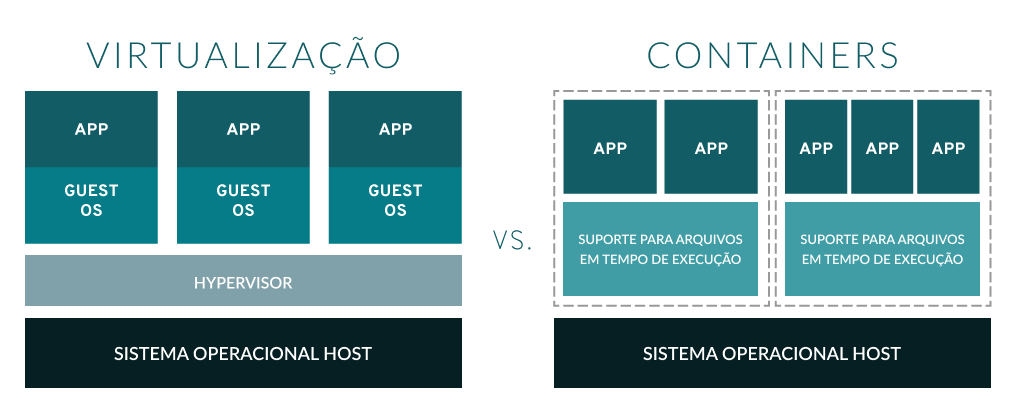
\includegraphics[width=.80\textwidth]{assets/virtualization-vs-containers.png} 
  \caption{Comparação entre o modelo de virtualização e modelo de containers (Adaptada de \cite{redhat2020Containers}).}
  \label{fig:virtualization-vs-containers}
\end{figure}

% Referencias
% - https://www.opservices.com.br/o-que-e-docker/
% - https://www.meupositivo.com.br/panoramapositivo/container-docker/
% - https://www.treinaweb.com.br/blog/no-final-das-contas-o-que-e-o-docker-e-como-ele-funciona/

% ---
\subsection{Computação em Nuvem}
\label{fund:nuvem}
Há uma crescente demanda por serviços de Tecnologia em Informação, TI, ofertados através da Internet, incluindo armazenamento de dados, hospedagem de sites, softwares, banco de dados, rede entre outros. Este fornecimento de serviços de computação, via Internet, é chamado de computação em nuvem. Tal crescimento vem das diversas vantagens oferecidas pela computação em nuvem, como uma disponibilidade maior, recursos flexíveis, normalmente se pagando apenas o usado, trazendo assim, uma redução no custo, possibilidade de escalonamento de acordo com as necessidades da empresa, não precisar gastar nem se preocupar com a infraestrutura entre outras \cite{sousa2009computaccao}.

% ---
\section{Aplicativo Móvel}
\label{fund:app}
Aplicativo móvel, APP, é um \textit{software} desenvolvido especificamente para dispositivos móveis, como telefones celulares, tablets, relógios inteligentes entre outros. Cada SO utiliza uma determinada linguagem de programação para desenvolvedores poderem criar os apps. Com uma grande diversidade de sistemas operacionais, com linguagens de programação distintas, transformam o desenvolvimento de aplicativos multiplataformas mais trabalhoso e repetitivo, pois tem que ser programada uma versão diferente para cada plataforma. Tendo esse problema em mente, várias formas de programação híbridas foram criadas, com o princípio de poder programar utilizando apenas um código para várias plataformas distintas, dentre elas, as duas que mais se destacam atualmente são o Flutter e o React Native.

% ----
\subsection{React Native}
\label{fund:react-native}
O React Native é um \textit{framework} para desenvolvimento nativo voltado para dispositivos para os dois principais SO móveis atualmente, Android e iOS. Ele dispõe de um código aberto, mantido pelo Facebook e sua comunidade. É um \textit{framework} bastante popular, utilizado por grandes empresas globais atualmente, como Netflix, Uber, a própria Facebook e empresas brasileiras como o EBANX e a Globo \cite{empresasbrreact}.

O React Native utiliza a linguagem JavaScript como principal e a renderiza para código nativo, para isso é adicionado uma camada em JavaScript, chamada de \textit{Bridge} que se comunica com o sistema operacional, mandando comandos para renderizar os componentes nativos \cite{docreactnative}.

% ---
